	% !TEX encoding = UTF-8 Unicode
% !TEX program = pdflatex
% !TEX spellcheck = en_US


% In order to correctly compile this document,
% execute the following commands:
% 1. pdflatex
% 2. pdflatex
% 3. pdflatex



\documentclass[amsthm,ebook]{saparticle}

% IF YOU USE PDFLATEX
\usepackage[utf8x]{inputenc}
% if you write in english and in greek
\usepackage{ucs}
\usepackage[greek,english]{babel}
\languageattribute{greek}{polutoniko}

% IF YOU USE XELATEX
%\usepackage{polyglossia}
% if you write in italian
%\setmainlanguage{italian}
% If you want put some ancient greek:
%\setotherlanguage[variant=polytonic]{greek}
%\newfontfamily{\greekfont}[Ligatures=TeX]{Palatino Linotype}

% dummy text (remove in a normal thesis)
% remove if not necessary
\usepackage{siunitx}
%Natbib for bibliography management
\usepackage[authoryear]{natbib}
% custom commands
\newcommand{\bs}{\textbackslash}

%%%%%%%%
%TITLE:%
%%%%%%%%

\title{The Digital Edition of the Archaic Latin Inscriptions (7th{}-5th century B.C.)}
\author[unimi]{Giovanna Rocca }
\author[kore]{Giulia Sarullo \corref{first}}
\author[unimi]{Marta Muscariello}
\address[kore]{Università degli Studi di Enna "Kore"}
\address[unimi]{Università IULM Milano}
\cortext[first]{Corresponding author. Email: giulia.sarullo@unikore.it}
\date{2015-09-18}
\begin{document}


\maketitle
\begin{abstract}
This project consists in the digital edition of the archaic Latin inscriptions (7th – 5th century B.C.) according to the
EpiDoc Guidelines. The edition is the result of an autoptical examination of the epigraphic documents and of the
text-bearing objects, together with the analysis of previous studies. In the particular case of the Forum inscription,
this led to new discoveries and confirmed old hypotheses. Each text will be presented in an epigraphic chart, enriched
by photos and illustrations.\footnote{Giovanna Rocca (GR) is responsible for § \ref{sec:generalia} and \ref{sec:news};
Giulia Sarullo (GS) is responsible for § \ref{sec:3chart} and Marta Muscariello (MM) for § \ref{sec:4tech}.}
\end{abstract}
\keywords{Archaic Latin Inscriptions, Latin Epigraphy, EpiDoc, Digital Humanities, Epigraphic Edition, Forum inscription.}







\section{\emph{Generalia} [GR]}\label{sec:generalia}


\noindent The project \emph{Iscrizioni Latine Arcaiche (ILA)} consists in the digital edition of the inscriptions found in old
\emph{Latium}\footnote{With the two exceptions of the \emph{Vendia's} Urn, found in Cerveteri, and the Garigliano bowl.}
dating back to the period between the 7th and the 5th century B.C. Between the end of the 19th century and the first
decades of the 20th century this \emph{corpus} consisted of only four inscriptions of a certain length, that is the \emph{Duenos}
vase (1880), the \emph{Fibula Praenestina} (1887), the \emph{Forum} inscription (1899) and the \emph{Tibur} pedestal inscription (1926),
besides other shorter but still very interesting texts that offered important cultural information (such as the
inscription from the \emph{Regia, REX, CIL} I$^2$ 479). In the second half of the 20th century, the \emph{corpus} grew significantly and
reached the total of about eighty documents that have not been gathered in a comprehensive edition yet. The updated
\emph{corpus} includes new and crucial discoveries, some of which have already been published in a traditional way (in print),
such as the inscriptions from \emph{Satricum} and the fragments found at the \emph{Palatinum}, whereas others are still unpublished,
as in the case of the recent findings from the \emph{Regia}. The quantitative and qualitative enrichment provided by recent
new readings of the texts and the new data emerged justify and require a new publication. 

Most of the inscriptions in the collection are \emph{frustuli} or single letters: these texts, though not really relevant from
the linguistic point of view, are important testimony of the use of writing in \emph{Latium} since the 7th century B.C. 

The website is then an absolute novelty in the field of digital epigraphy, since at the moment no online epigraphic
collection specifically dedicated to these documents exists. It is well known that, for every kind of publication, a
digital edition provides several advantages, for example: the possibility to update both the textual \emph{corpus} and the
bibliography continuously; the hypertextual structure, that allows the user to utilize the edition in different ways;
the opening to a public that is heterogeneous and wider than the one a work addressed to specialists can reach. In
which other ways can the web respond to the specific requirements of a peculiar \emph{corpus} such as ours with distinguishing
features, different from the later Latin epigraphy optimally reproduced in the \emph{Epigraphic Database Rome} (EDR)?

First of all, by using the EpiDoc encoding standard, which is compatible with other encoding systems, it will be
possible to transfer our data to EDR and to the EAGLE-Europeana Network (see Sec. \ref{sec:4tech}).

The hypertextual structure of the edition is surely one of its assets, in that it enables the user to find information
about each text (images, bibliographical references, etc.) immediately and consider the inscription in the context of
its place of finding; at the same time, it encourages a direct `in real time' comparison between texts. Moreover,
this kind of structure allows us to obviate the inconvenience of an edition that presents only a specifically
`historical', `archaeological' or `epigraphic' point of view, as sometimes happens in traditional
editions. This is achieved thanks to cross-references to topics analyzed in depth by specialists, thus making our
edition a useful research tool for various branches of learning.

Besides what has been illustrated so far, the presence of complex indexes, through which it will be possible to locate
the inscription from different starting points, will allow the user to search the texts according to various
parameters: dating, place of finding, object type, and textual type (see § \ref{sec:3chart}). 

The choice of the method to adopt as regards the interpretative transcription is problematic: it is clear that it is
absolutely impossible to be completely neutral or objective. Unlike the diplomatic transcription, for which a critical
apparatus can be constructed and be extremely useful, the same is not possible for the interpretative transcription: an
exhaustive critical apparatus would imply a superabundance of information that could negatively influence the
scientific nature and the usability of the edition, especially in the case of inscriptions that have been variously
interpreted since their discovery. For longer inscriptions (\emph{e.g.} \emph{Forum} Inscription, \emph{Duenos} vase, Tivoli inscription,
Garigliano bowl), the numerous readings that have been proposed so far by scholars have been compared and verified in
the light of linguistic criteria and of the new data in order to obtain an edition of the text that, although it cannot
be considered the definitive interpretation and does not solve all the pending issues, poses itself as a new starting
point for future research. A cross-reference to all the other interpretations will offer a complete source of
information and a tool that intends to be useful and exhaustive.

The archaic Latin inscriptions play a fundamental role in the study of the first stages of the language, since they
present particular features that allow us to investigate the various steps that led to ``standard Latin''. The language
attested in our inscriptions can be considered a \emph{Restsprache} insofar as it is not `readable' through later Latin
but it can be `interpreted'. The linguistic commentary will be carried out, \emph{in votis}, in the second phase of this
project. Here the research focuses on the epigraphic features, that show a plurality of forms and of alphabets in such
a limited \emph{corpus}. The chronological and geographical distribution of the signs and of the variants in use in the
inscriptions have been analyzed in order to offer valid elements to the study of the evolution of the alphabetic model
between the 7th and the 5th century B.C.

\section{Epigraphic News about the Forum Inscription [GR]}\label{sec:news}


\noindent Thanks to the agreement and collaboration with public authorities, we were invited to take part in an extraordinary
event (July 3rd 2015), that is the 3D laser scanning of the Forum Cippus (CIL I$^2$, 1).\footnote{Cippus of tuff found
under the \emph{Lapis Niger} by Giacomo Boni in 1899. The inscription is cut boustrophedon on the four faces of the pillar and
on the edge sliced between face D and face A. The stone (late 6th B.C.) is badly damaged in the upper part so that the
beginnings and the endings of the lines are lost. The text has been interpreted as a sacred law.} The autopsy, carried
out with the help of a strong source of light, and the observation of the scanning in real time clarified, hopefully in
a definite way, some controversial issues about the presence of dividing signs on face A and, at the same time, opened
a new perspective on the reading of line 16 (face E). 

One of the epigraphic problems concerning this inscription consisted in the absence of punctuation on face A, in
comparison with the other faces in which three vertical dots divide the syntactical units. This lack was particularly
suspicious in a sequence in which there are no exegetical alternatives (SAKROSESED = \emph{sakros esed}). As a consequence,
scholars tried to find an explanation for this absence: the inscription was carved by different hands; the inscription
was made up of different texts, each copied from different drafts; the antigraph was in \emph{scriptio continua} and the
inscriber was not familiar with this procedure; the punctuation was not accurately assigned.

As a matter of fact, face A conforms to the others, showing three vertical dots after \emph{sakros} and also, although less
deep and more worn-out, after \emph{esed}\footnote{The details of significant portions of the inscriptions will be shown on
the website with several photographs. } (Fig.~\ref{fig:1}). This fact was highlighted by \citet{gamurrini_paleografia_1899} and the three dots
appear in the apograph in \citet[col. 1003]{hulsen_neue_1899},  and they could also be guessed in the photograph Anderson 3192
(Archivio Alinari). Nevertheless, the \emph{post} \citet{goidanich_rapporti_1943} \emph{vulgata} and the difficulties in checking in person the
stone, because of its almost unreachable and scarcely illuminated position that led to the publication of studies not
supported by an autoptical check, perpetuated a reading influenced by the uncertainty in distinguishing between natural
cavities or notches due to the nature of the stone and `significant' holes caused by the tool used for writing. 

\begin{figure}[!bp]
\centering
 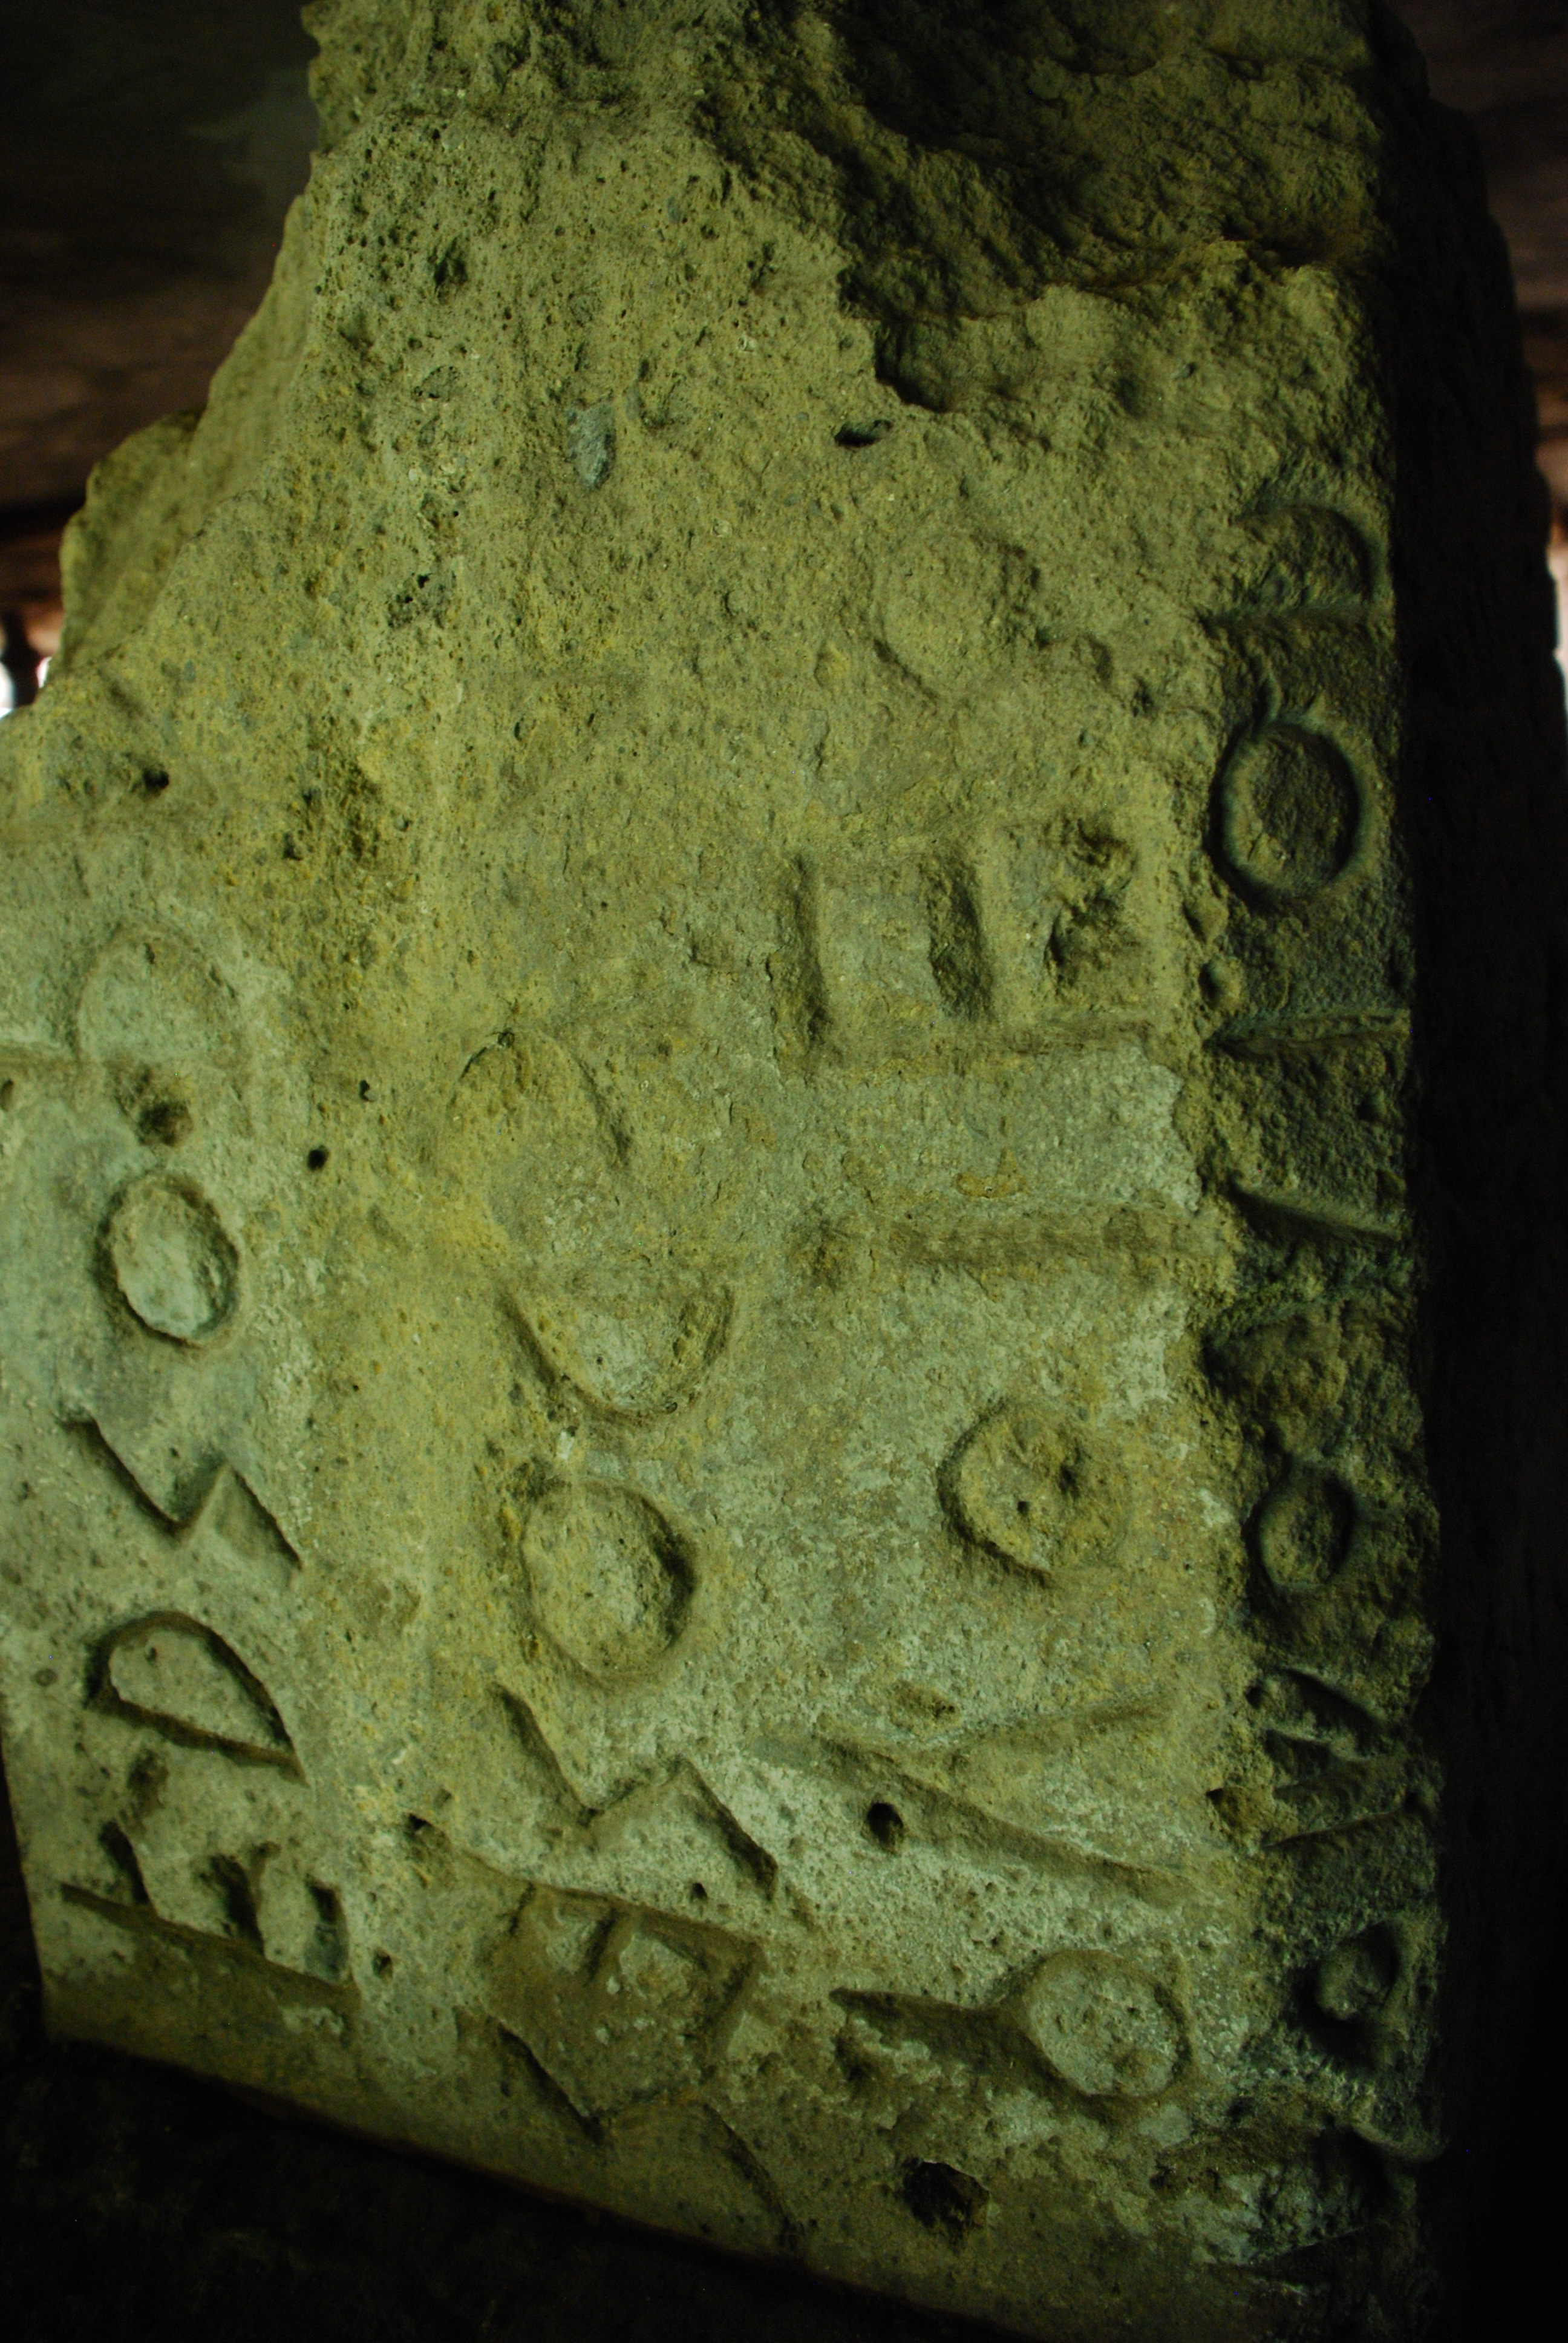
\includegraphics[width=\columnwidth]{IscrizioniLatineArcaicheEAGLE2016-img001.png}
\caption{Forum Cippus, Face A and Face E (by Marta Muscariello).}
\label{fig:1}
\end{figure}





The most relevant news arrives from the analysis of line 16 (face E). This has been read up to now as \emph{loiuquod()qo}
\citep{wachter_altlateinische_1987}, \emph{loi\{u\}quiod} \citep{_studies_1993}, \emph{LOIUQUIOD[QO}] \citep{baldi_foundations_2002}, \emph{LOIUQUIOD,QO///} \citep{hartmann_fruhlateinischen_2005},\footnote{The
final \emph{QO} is based only on \citet{goidanich_rapporti_1943}.} in order to explain the `unusual' shape of \emph{V} (letter no. 4) that has
been recently read as \emph{F} \citep{prosdocimi_roma_2010}. As the scanning showed, the first vertical stroke, read as an \emph{I}, is much
closer to the sign that looks like a \emph{V} than it appears on the apographs and the photographs published so far;
especially shots taken from an oblique and not a frontal point of view can be misleading. 

This point can result fundamental in understanding how the inscriber worked on the stone and how he corrected the
sign.\footnote{Other corrections can be found on the last line of face C (\emph{kapia} on \emph{kapa}) and on the second line of face
D where a \emph{V} was corrected into a \emph{koppa}. } Hypothesis no. 1 (which is also the simplest one): the sequence to write was
\emph{LOIVQVIOD} but, after he cut a first vertical stroke, the inscriber mistakenly started to cut the oblique stroke of a \emph{V}
instead of a second vertical stroke that would begin the V; he recognized the error and cut a vertical stroke next to
the first one and finally another oblique stroke that reached the bottom of the second vertical stroke, completing the
\emph{V}. Hypothesis no. 2 presumes the same order in cutting the strokes, but for a different reason: the sequence to write
was \emph{LOVQVIOD}, the inscriber started cutting the first stroke but he found an obstacle (\emph{i.e.} a hole in the stone), so he
continued with the oblique stroke on the right (thinner than the others) but he changed his mind and cut a second
vertical stroke close to the first one and joined it with a new oblique stroke. The short inner stroke has been
considered as a correction, \emph{i.e}. a deletion, and caused the expunction of the whole letter or its reading as an \emph{F}; as a
matter of fact, it is nothing else but the result of a first try to cut the oblique stroke. Of course, we could be more
precise after we receive the outcomes of the scanning, that will be ready soon. The following sign (nr. 4 or 5,
depending on the reading), instead, is surely a \emph{koppa} and not an \emph{O}.

Our reading proposal has the advantage of illustrating the sequence of the inscribing but does not solve the
interpretative problems: a \emph{louquiod} instead of a \emph{loiuquiod} / \emph{loiquiod} (for which \emph{lucus}, \emph{eloquium}, \emph{licium} and \emph{liquidus}
have been proposed) still needs to be explained and both still await a solution. 

\section{The Epigraphic Chart [MM]}\label{sec:3chart}


\noindent In the website, each text of the ancient Latin \emph{corpus} is presented by an \emph{ad hoc} designed chart in order to meet the
peculiar requirements of this kind of \emph{corpus}. The chart is organized in items that concern every important aspect
regarding the material and cultural contextualization of the inscription, from the archaeological support to the
epigraphic features. Such a detailed scheme contributes to making our project a research tool both as a complete source
for information retrieval and as an updated starting point for the study of the texts and of the language.

In this initial phase of \ Latin literacy, the linguistic data are not sufficient to establish the linguistic features
of this language – the \emph{corpus} chiefly consists of \emph{hapax}. As a consequence, the contextual data of the inscribed object
results being of great help to comprehend the text. For example, the new archaeological data found during the recent
excavation campaign in the \emph{Comitium} carried on under the direction of P. Fortini are providing helpful information for
the study of the Forum Inscription; in the past, the collection of all the fragmentary instrumental Latin inscriptions
up to the 4th century B.C. published by G. Colonna in 1980\footnote{In \citet{stibbe_lapis_1980}.} supplied, at least
partially, the extent of the alphabetization developing in \emph{Latium Vetus}, subtracting the major inscriptions from a sort
of ``documental isolation''; moreover, the data concerning the interaction with other inscriptions of ancient Italy are
fundamental, since these are different in languages and alphabets: besides the Etruscan examples in Rome, we can
remember the case of \emph{Satricum}, where both Latin and Volscan are attested,\footnote{See \citet[189-198]{rocca_i_1995}.} or the
Garigliano bowl which bears, together with the Latin inscription engraved inside, an inscription in Italic alphabet and
language on the external body of the vase,\footnote{On the relationship between the two inscriptions, see \citet{antonini_osservazioni_2012}.} that has also given a hint for a particular interpretation of the Latin text. 

The first item of the chart contains the ID tag assigned to the inscription in the ILA project, that identifies the text
with the find-spot (using the ancient place name whenever possible) followed by a progressive number: for example, the
\emph{Tibur} pedestal inscription (\emph{CIL} I$^2$ 2658) is denominated ``Tibur 1'', the inscription on the Garigliano bowl is called
``Garigliano 1''. Given the small number of find-spots, we decided to use the full name of the place, instead of
abbreviations; possible new findings that could emerge in the future from the same site will be easily added to the
corpus simply by increasing the number. Beside the ID tag attributed to the inscription we quote the most common names
attributed to the object, stratified in time in literature and well known to the scholars (for example ``\emph{Duenos} vase'' /
``Vase of the Quirinal''). We then indicate here, in the item `Present collocation', where the inscription is
preserved with, when possible, the inventory number.

The chart continues with a group of three items that form the section dedicated to the `Archaeological data': the
‘Description of the object' (with the general type, the possible peculiar features, the function and the dimensions of
the inscribed object); the ‘Provenance' (that is the place where the object was found and its exact archaeological
context);\footnote{In the case of mobile objects a different place of fabrication can be presumed, as in the case of the
\emph{Vendia}'s Urn, found in Cerveteri, but considered by some to have been fabricated somewhere else in \emph{Latium}.} the
‘Date', which quotes the hypotheses given by scholars about the chronological coordinates of the inscription.
Concerning this item, we must keep in mind that the dating of the \emph{antiquissimae} is often approximate, and it is based
on different criteria (at times archaeological, at others epigraphic or linguistic or with convergences of two or of
all these factors); in some cases, the gap is so wide to almost seem fluctuant depending on which criterion is
considered. Without doubt this long-standing problem must be held in consideration, also remembering that for some
inscriptions a chronological lowering to the 4th or even the 3rd century B.C. has been proposed. The difficulty in
dating the objects and the rarity of the findings is surely connected to the difficulty in defining the specific
features of the language testified by these inscriptions.\footnote{On the periodization of Latin, P. Cuzzolin and G.
Haverling state: ``The division of the history of a language into different periods implies that we have a rather clear
picture of what language we have dealing with. At two points in the history of Latin we are not quite sure of this: the
exact moments in which Latin is born and in which it is transformed into Romance are not easily determined. The problem
is to determine what is Latin and what is not: unfortunately there is no overall agreement on whether all of the early
inscriptions considered to provide us with early examples of Latin actually do that.'' \citep[20]{cuzzolin_syntax_2009}.}

The charts present several photographs of the inscriptions, taken during the photographic campaign carried out by the
project's team. Enlargements of some useful or problematic details of the inscription have been added: the richness in
images is related to the participation of the project in the Europeana network, a database of images of the European
cultural heritage. Although the images illustrate the inscription in an optimal way, fac-similes of each text will also
be provided, clearly related with the transcription provided by the editor. 

We offer two kinds of transcription, the ‘Diplomatic transcription' and the ‘Interpretative transcription', which
provides the edition of the text. The need for a diplomatic transcription is due to the problematic nature of archaic
texts: in the case of the \emph{Duenos} vase, as it is well known, the second section of the text is almost always given by
scholars in diplomatic transcription because of the difficulties in segmenting the phrases into words (but with
attempts of interpretations of small portions). 

In the item `Textual typology' inscriptions are classified according to the nature of the text, taking into due
consideration the peculiarities of this \emph{corpus}. In the chronological span between the 7th and the 5th century B.C. the
codification of formularies both of possession and of gift/dedication is still \emph{in fieri} in the various linguistic
branches spoken in ancient Italy (with the exception of Greek); for this reason, from a classificatory point of view an
inscription can be ‘anomalous' in two ways: on the one hand, it can lack the typical elements of a formulaic scheme
that will be fixed later on, thus requiring a further interpretative effort in order to assign it to a specific textual
category; or, on the other hand, it can result more complex than the standard formula and present elements that can be
related to more than one textual typology: in this case, the object type and the archaeological context are determinant
for the overall classification.\footnote{On this subject, see two recent publication, \citet{poccetti_paradigmi_2009} and \citet{maras_storie_2015}.} 

A further group of items composes the ‘Epigraphic data' section: the analysis begins from the ‘Position of the
inscription' on the object, which indicates the relationship between the text and the inscribed object, an aspect that
has important consequences on the function and the fruition of the inscription.\footnote{An important methodological
point was established by \citet{susini_epigrafia_1982}.} We then have ‘Scriptura', where the execution technique is described;
‘Direction of writing', \emph{i.e.} right-to-left, left-to-right, \emph{boustrophedon}, etc.; ‘Dividing signs', in which the presence
of punctuation and its eventual function is signaled; ‘Dimensions of the letters', which is important as regards the
visibility of the inscription in relation with the object and the observer. This section ends with the ‘Epigraphic
commentary', containing the description and analysis of the letters one by one both from the formal (shape-model of the
letter) and the factual point of view (possible particular features in the execution of the inscription) and some
general observations.

The ‘Notes and issues' item gathers historical-bibliographical notes, observations and discussions on the most
problematic points of each inscription: the insertion of the discussion at the end of the chart offers the advantage of
having all the basic information on the object and on the inscription immediately available, while the study in depth
of the issues that deserve a thorough analysis is treated in a separate section. 

The chart is closed by the ‘Bibliography' section. The ‘\emph{Editio princeps}' and the possible ‘First notice' (if the
inscribed object had been mentioned in a publication preceding the first edition of the text) are indicated in two
separate items. Then the complete bibliography of the inscription follows in chronological order, from the most dated
to the most recent publications; the chronological order, in comparison with the alphabetical one, allows us to find
more easily the latest works on the inscriptions or those published in a certain period in the history of the studies. 

\section{Technical notes [GS]}\label{sec:4tech}


\noindent An epigraphic \emph{corpus} can be digitalized in different ways, according to the specific issues that each project intends to
tackle. Unlike EDR that, as t	he other projects constituting the \emph{Electronic Archive of Greek and Latin Epigraphy}
(EAGLE),\footnote{\url{http://www.eagle-eagle.it/}. The other databases related to EAGLE are the Epigraphic Database Bari
(EDB), \url{http://www.edb.uniba.it/}, the Epigraphische Datenbank Heidelberg (EDH),
\url{http://edh-www.adw.uni-heidelberg.de} and Hispania Epigraphica (HE),
\url{http://www.eda-bea.es/}.} is a database, the archaic Latin inscriptions have been digitalized according to the EpiDoc
Guidelines.\footnote{For further information on EpiDoc and its history, see \citet{Elliot:2006aa}.
The guidelines are available at \url{http://www.stoa.org/epidoc/gl/latest/}.} This is a set of specifications and encoding
tools in XML (\emph{eXtensible Markup Language}) for the scientific edition of ancient texts based on the \emph{Text Encoding Initiative} (TEI), a set of XML specifications designed for the digital publication of texts and manuscripts for
research purposes.\footnote{\url{http://www.tei-c.org/index.xml}. See also \citet{Consortium:2008aa} (About these Guidelines):
``The TEI encoding scheme is of particular usefulness in facilitating the loss-free interchange of data amongst
individuals and research groups using different programs, computer systems, or application software''.} EpiDoc is
becoming more and more a point of reference for digital epigraphic projects\footnote{On the relationship between EAGLE
projects and EpiDoc see \citet{felle_esperienze_2012}.} and it is also the standard chosen for the aggregation of the archives' data in
the recently constituted network, again called EAGLE (\emph{Europeana Network of Ancient Greek and Latin
Epigraphy}),\footnote{\url{http://www.eagle-network.eu}. About the new \emph{Best Practice Network}, co-founded by the European
Commission, see \url{http://www.europeana.eu}.} in which, besides the data of the EAGLE archives, the archaic Latin
inscriptions \emph{corpus} will also converge. As a matter of fact, inscriptions encoded with EpiDoc are not only compatible
with other projects created according to these Guidelines, but they can also be transferred from a system into another
without losing any information; actually, since XML consists in a semantic markup, that is related to the content of
the information and not to its appearance, it is possible to modify the look of the final result by simply operating on
the style sheet,\footnote{In XML, all information related to the formatting of the text are registered on a separate
file called style sheet, see \citet[104, 110-111]{bodard_epidoc:_2009}.} not having to revise the single files. This will facilitate
the integration of the archaic Latin inscriptions into wider digital collections such as EDR and EAGLE-Europeana.
Moreover, since the file thus encoded can also be translated into another markup language, their survival despite any
future technical evolution is guaranteed.\footnote{\citet[37-38]{tissoni_epidoc_2008} and \citet[104-105]{bodard_epidoc:_2009}.}

Furthermore, the XML edition of an inscription (or of an entire \emph{corpus}) created according to the EpiDoc Guidelines will
produce a digital edition of the text that complies to Leiden Conventions\footnote{On Leiden Conventions, the standard
used to annotate epigraphic documents and papyri in printed editions, see \citet{krummrey_criteri_1980}, \citet{panciera_segni_2006} and \citet{panciera_i_2006}. About their use in EpiDoc's files see \citet{elliot_conformance_2007}, \citet[229]{burnard_electronic_2006} and \citet[105]{bodard_epidoc:_2009}.} that will show the
same typographical marks a printed edition following the Leiden system would have, thus being immediately
comprehensible to any epigrapher.

The archaic Latin inscriptions pose various epigraphic problems, related to their antiquity, that require specific
solutions also with regard to the markup. Since the EpiDoc Guidelines were originally conceived to encode in XML later
epigraphic documents, it has been necessary to adapt these Guidelines to respond to the peculiar issues of this
\emph{corpus}.\footnote{See \citet[162-167]{sarullo_ledizione_2011}, where a few examples of markup are quoted. } For this reason, some elements
have been adapted and others have been specially designed, and this was possible thanks to the fact that XML is an
extensible system.

The major encoding issues concern the rendering of the direction of writing and of reversed and upside-down letters.
Unlike later texts, predominantly left-to-right, the inscriptions of the ILA \emph{corpus} show a certain degree of
fluctuation in the direction of writing. Besides left-to-right, right-to-left and boustrophedic inscriptions, there are
also some particular cases, such as the lamina from Lavinium (CIL I$^2$ 2833) and the Tibur pedestal inscription (CIL I$^2$
2658), that requires a specific treatment. For these texts, it was necessary to adopt the \texttt{{\textless}lb
rend={\textquotedbl}up-to-down{\textquotedbl}{\textgreater}} and \texttt{{\textless}lb
rend={\textquotedbl}down-to-up{\textquotedbl}{\textgreater}} elements in order to render the peculiar directions in
which the text was cut.\footnote{The issue of the direction of writing was the subject of much debate at the 6th EAGLE
International Event \emph{Off the beaten track. Epigraphy at the borders} (Bari, September 24th{}-25th, 2015). The discussion
highlighted how this is a matter of great relevance both for the archaic inscriptions and the testimonies from late
antiquity and the necessity to establish a common standard to encode the instances of ``non-standard'' directions of
writing emerged. For this reason, this issue will surely be the object of further consideration in the future.}
Reversed and upside-down letters are usually left unmarked in traditional epigraphic editions and we decided to comply
to this practice. Nevertheless, the \texttt{{\textless}hi{\textgreater}} element has been used to mark up these letters, with
two different values of @rend. For reversed letters, the \texttt{{\textless}hi
rend={\textquotedbl}reversed{\textquotedbl}{\textgreater}} was used, a tag that in the EpiDoc Guidelines is used to
encode the \emph{litterae inversae}, enclosed in double round parentheses, such as in ((C)) for mulier.\footnote{See \citet[1722]{panciera_i_2006}.} For upside-down letters, a new value was provided, \texttt{{\textless}hi
rend={\textquotedbl}upside-down{\textquotedbl}{\textgreater}}, since none of the allowed values of \texttt{@rend} for the
\texttt{{\textless}hi{\textgreater}} element is suitable for this issue.

XML also allows us to encode the semantic structure of the texts. This kind of markup does not influence how the text is
displayed but it is essential to generate the \emph{Index verborum} and to allow a word-based search within the \emph{corpus}. The
antiquity of the documents compelled to index the words as they appear in the inscription, because in most of the cases
a lemmatization would be forcing; for the same reason, some sequences that remain difficult to interpret were not
segmented and the search for a portion of text will be possible. 

Finally, the EpiDoc file contains all information about the text-bearing object (description, dating) and the text
(critical apparatus, commentary); the encoding of these data allows us to generate the indexes that, together with the
bibliographical references and the images, enrich the digital edition and make the utilization of the text more
complete. 

\nocite{colonna_iscrizioni_2007}
\bibliographystyle{sapauth-eng}
\bibliography{../../EAGLE}

\end{document}
